\documentclass{standalone}
\usepackage{tikz}
\begin{document}
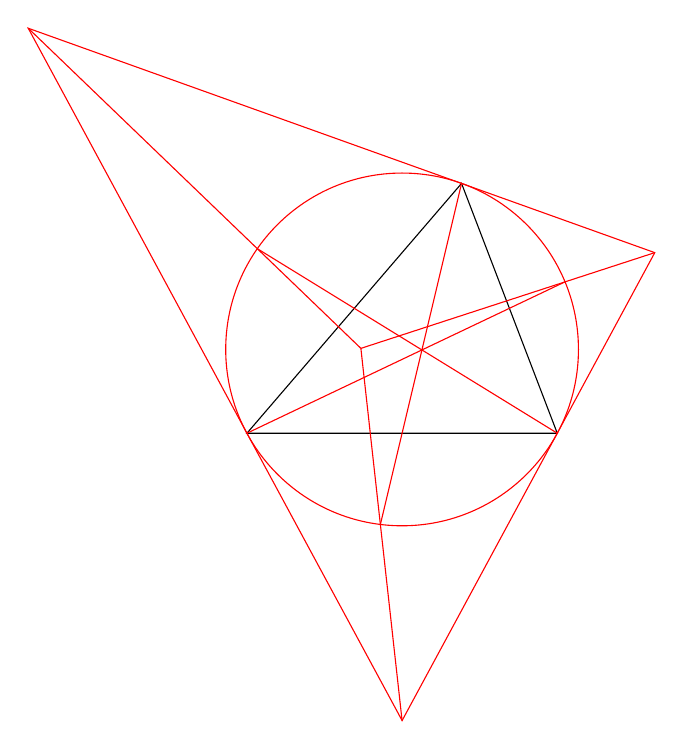
\begin{tikzpicture}[x=1pt,y=1pt]
\draw (181.41,-76.67) -- (103.86,-166.94) -- (216.00,-166.94) -- cycle;
\draw[red] (159.92,-136.65) circle (63.73);
\draw[red] (24.83,-20.59) -- (251.23,-101.68) -- (159.93,-270.76) -- cycle;
\draw[red] (181.41,-76.67) -- (152.08,-199.90);
\draw[red] (103.86,-166.93) -- (218.79,-112.24);
\draw[red] (216.00,-166.93) -- (107.62,-100.25);
\draw[red] (24.83,-20.59) -- (145.04,-136.27);
\draw[red] (159.92,-270.76) -- (145.03,-136.26);
\draw[red] (251.23,-101.68) -- (145.04,-136.27);
\end{tikzpicture}
\end{document}
